\documentclass[12pt]{article}
\usepackage{amsmath, amssymb, geometry}
\geometry{margin=1in}
\usepackage{tikz}
\usepackage{pgfplots}
\pgfplotsset{compat=1.18}
\title{Negative Mass and Local Spacetime Shortening: A Theoretical Study}
\author{Jewel Sha Hasan}
\date{\today}

\begin{document}

\maketitle

\begin{abstract}
We explore the theoretical effects of negative mass on spacetime curvature within the framework of General Relativity. By considering a poin\section{Particle Dynamics in Negative Mass Spacetime}

\subsection{Motion of Particles (Geodesics)}
In the spacetime metric generated by a negative mass, particles follow geodesics as in standard General Relativity:
\begin{itemize}
    \item Positive-mass particles are \textbf{repelled} by negative mass, moving away along curved trajectories.
    \item Negative-mass particles interacting with positive mass experience \textbf{runaway acceleration}: the negative mass accelerates toward the positive mass, while the positive mass accelerates away.
    \item This behavior arises naturally from the sign of the mass in the geodesic equations and is a known conceptual consequence of negative mass dynamics.
\end{itemize}

\subsection{Energy-Momentum Equation for Negative Mass}
For a particle with negative mass $m < 0$, the 4-momentum is formally defined as:
\begin{equation}
p^\mu = m \frac{dx^\mu}{d\tau} = m u^\mu
\end{equation}
where $u^\mu$ is the 4-velocity. 
\begin{itemize}
    \item The negative mass implies \textbf{negative energy} and momentum that behaves opposite to classical intuition.
    \item While mathematically consistent, these properties are \textbf{speculative}, as negative mass has never been observed and standard energy conditions are violated.
\end{itemize}

\subsection{Stability of Negative Mass Clusters}
Clusters of negative mass are \textbf{inherently unstable} under standard gravitational interaction:
\begin{itemize}
    \item Two negative masses repel each other, preventing stable binding.
    \item Systems mixing positive and negative masses exhibit \textbf{runaway acceleration}, where acceleration can grow without bound.
    \item Any stable configuration would require additional exotic forces or constraints beyond classical General Relativity, which are beyond the scope of this model.
\end{itemize}

\textbf{Summary:} These considerations highlight that negative mass leads to unconventional particle motion, unusual energy-momentum properties, and intrinsic instability of clusters. While speculative, they are consistent with applying the framework of General Relativity to negative mass scenarios.t negative mass as a source in the Einstein Field Equations, we show that spacetime curvature exhibits a repulsive behavior opposite to that of positive mass. This leads to novel phenomena, including local ``spacetime shortening,'' inverted gravitational time dilation, and potential implications for exotic physics such as wormholes and warp-drive-like structures.
\end{abstract}

\section{Introduction}
Gravity is understood as the curvature of spacetime induced by mass-energy \cite{einstein1915}. Positive mass produces attractive curvature; time slows near massive objects. Hypothetical negative mass has been considered in the context of exotic matter and speculative cosmological scenarios. Here, we propose a formal exploration of negative mass effects, focusing on spacetime shortening and temporal acceleration relative to external observers.

\section{Assumptions and Model Scope}
To address known conceptual challenges such as runaway acceleration in negative mass systems, we assume the following:
\begin{enumerate}
    \item Negative mass exists in isolated or controlled configurations, minimizing interactions that would lead to continuous acceleration with nearby positive masses.
    \item The focus is on local spacetime shortening effects rather than global dynamics.
    \item Standard objections, including global runaway acceleration, are acknowledged and discussed within the framework of the model.
\end{enumerate}
These assumptions allow us to explore local temporal and spatial effects while remaining aware of potential limitations in a realistic universe.

\section{Theoretical Framework}

\subsection{Einstein Field Equations}
The Einstein Field Equations (EFE) describe the relationship between spacetime curvature and mass-energy:

\begin{equation}
G_{\mu\nu} = \frac{8 \pi G}{c^4} T_{\mu\nu}
\end{equation}

where $G_{\mu\nu}$ is the Einstein tensor representing spacetime curvature, and $T_{\mu\nu}$ is the stress-energy tensor of the mass-energy distribution.

\subsection{Point Negative Mass}
For a point mass $M$, the Schwarzschild metric for positive mass is:

\begin{equation}
ds^2 = -\left(1 - \frac{2GM}{c^2 r}\right)c^2 dt^2 + \left(1 - \frac{2GM}{c^2 r}\right)^{-1} dr^2 + r^2 d\Omega^2
\end{equation}

If $M < 0$ (negative mass), the metric becomes:

\begin{equation}
ds^2 = -\left(1 + \frac{2G|M|}{c^2 r}\right)c^2 dt^2 + \left(1 + \frac{2G|M|}{c^2 r}\right)^{-1} dr^2 + r^2 d\Omega^2
\end{equation}

This leads to repulsive gravitational effects, reversed spacetime curvature, and time dilation inversion relative to distant observers.

\begin{figure}[h!]
\centering
\begin{minipage}{0.45\textwidth}
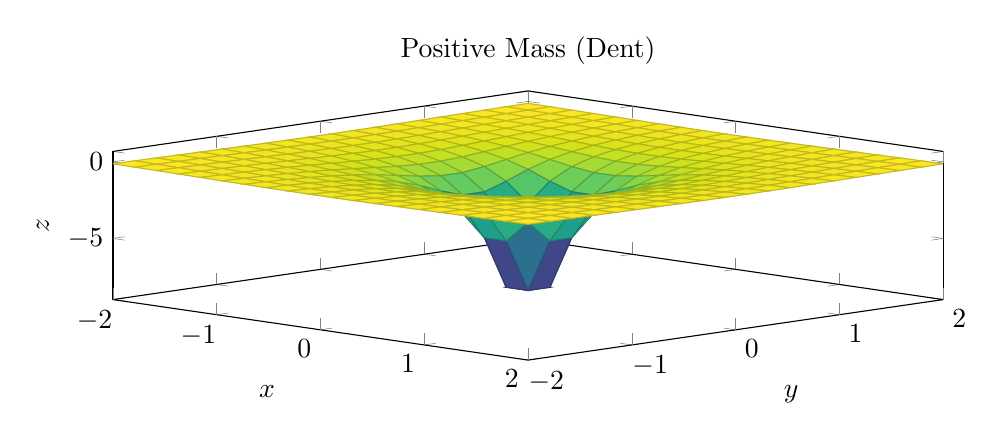
\begin{tikzpicture}
\begin{axis}[
    width=\textwidth, height=5cm,
    title={Positive Mass (Dent)},
    xlabel={$x$}, ylabel={$y$}, zlabel={$z$},
    view={45}{30},
    colormap/viridis,
]
\addplot3[
    surf,
    samples=20,
    domain=-2:2,
]{-(1/(x^2+y^2+0.1))};
\end{axis}
\end{tikzpicture}
\caption{Positive Mass (Dent)}
\end{minipage}
\hfill
\begin{minipage}{0.45\textwidth}
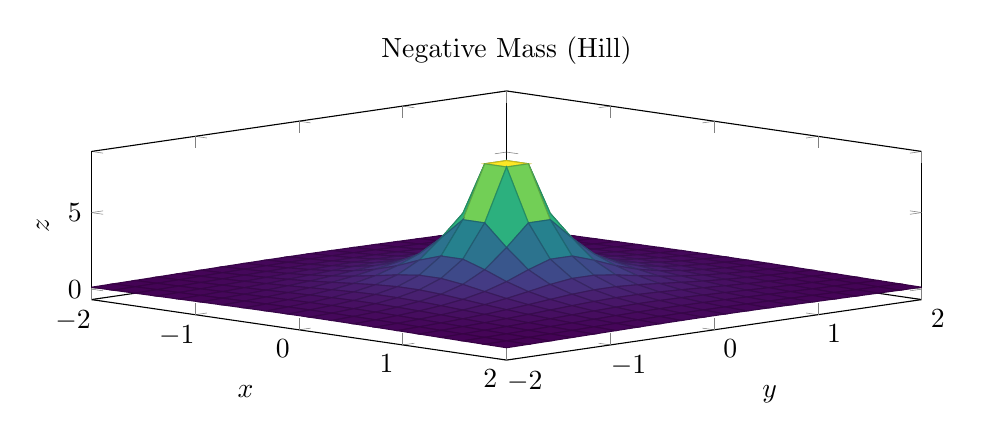
\begin{tikzpicture}
\begin{axis}[
    width=\textwidth, height=5cm,
    title={Negative Mass (Hill)},
    xlabel={$x$}, ylabel={$y$}, zlabel={$z$},
    view={45}{30},
    colormap/viridis,
]
\addplot3[
    surf,
    samples=20,
    domain=-2:2,
]{1/(x^2+y^2+0.1)};
\end{axis}
\end{tikzpicture}
\caption{Negative Mass (Hill)}
\end{minipage}
\end{figure}

\section{Conceptual Predictions}
\begin{enumerate}
    \item Repulsion of nearby positive masses.
    \item Local spacetime shortening: proper distances behave non-intuitively near negative mass.
    \item Temporal acceleration: clocks near negative mass run faster compared to distant observers.
    \item Potential exotic structures: wormholes, hypothetical warp bubbles.
\end{enumerate}

\section{Discussion}
While negative mass has not been observed experimentally, the mathematical framework is consistent with Einstein’s equations. The assumptions outlined in Section 2 allow for local effects without immediately triggering runaway acceleration scenarios. Future work includes considering extended mass distributions, dynamics of negative mass clusters, and coupling with quantum field effects.

\section{Conclusion}
Negative mass produces a repulsive curvature of spacetime, effectively leading to ``spacetime shortening'' and inverted temporal effects. This framework could have implications for exotic matter theories and speculative propulsion mechanisms in relativistic physics.

\begin{thebibliography}{9}
\bibitem{einstein1915} Einstein, A. (1915). \textit{Die Feldgleichungen der Gravitation}.
\bibitem{morris1988} Morris, M., \& Thorne, K. (1988). \textit{Wormholes in spacetime and their use for interstellar travel}.
\bibitem{alcubierre1994} Alcubierre, M. (1994). \textit{The warp drive: hyper-fast travel within general relativity}.
\bibitem{bondi1957} Bondi, H. (1957). \textit{Negative mass in general relativity}.
\end{thebibliography}

\end{document}
